\documentclass{beamer}
\usepackage[utf8]{inputenc}

\usetheme{Madrid}
\usecolortheme{default}
\usepackage{amsmath,amssymb,amsfonts,amsthm}
\usepackage{txfonts}
\usepackage{tkz-euclide}
\usepackage{listings}
\usepackage{adjustbox}
\usepackage{array}
\usepackage{tabularx}
\usepackage{gvv}
\usepackage{lmodern}
\usepackage{circuitikz}
\usepackage{tikz}
\usepackage{graphicx}

\setbeamertemplate{page number in head/foot}[totalframenumber]

\usepackage{tcolorbox}
\tcbuselibrary{minted,breakable,xparse,skins}



\definecolor{bg}{gray}{0.95}
\DeclareTCBListing{mintedbox}{O{}m!O{}}{%
  breakable=true,
  listing engine=minted,
  listing only,
  minted language=#2,
  minted style=default,
  minted options={%
    linenos,
    gobble=0,
    breaklines=true,
    breakafter=,,
    fontsize=\small,
    numbersep=8pt,
    #1},
  boxsep=0pt,
  left skip=0pt,
  right skip=0pt,
  left=25pt,
  right=0pt,
  top=3pt,
  bottom=3pt,
  arc=5pt,
  leftrule=0pt,
  rightrule=0pt,
  bottomrule=2pt,
  toprule=2pt,
  colback=bg,
  colframe=orange!70,
  enhanced,
  overlay={%
    \begin{tcbclipinterior}
    \fill[orange!20!white] (frame.south west) rectangle ([xshift=20pt]frame.north west);
    \end{tcbclipinterior}},
  #3,
}
\lstset{
    language=C,
    basicstyle=\ttfamily\small,
    keywordstyle=\color{blue},
    stringstyle=\color{orange},
    commentstyle=\color{green!60!black},
    numbers=left,
    numberstyle=\tiny\color{gray},
    breaklines=true,
    showstringspaces=false,
}
\title{2.10.85}
\date{17th September, 2025}
\author{Puni Aditya - EE25BTECH11046}

\begin{document}

\frame{\titlepage}
\begin{frame}{Question}
Let $\vec{P}$ be the plane $3x + 2y + 3z = 16$ and let 
$S : \alpha \hat{i} + \beta \hat{j} + \gamma \hat{k},\text{ where } \alpha + \beta + \gamma = 7$
and the distance of $\brak{\alpha, \beta, \gamma}$ from the plane is $\frac{2}{\sqrt{22}}$.
Let $\vec{u}, \vec{v}, \vec{w}$ be three distinct vectors in $S$ such that $|\vec{u} - \vec{v}| = |\vec{v} - \vec{w}| = |\vec{w} - \vec{u}|$. Let $V$ be the volume of the parallelepiped determined by vectors $\vec{u}, \vec{v}, \vec{w}$. Then the value of $\frac{80}{3} V$ is
\rule{1cm}{0.1pt}.
\end{frame}

\begin{frame}{Theoretical Solution}
Let the matrix of vectors be 
\begin{align}
	\vec{A} = \myvec{\vec{u} & \vec{v} & \vec{w}}
\end{align}
The volume 
\begin{align}
V = \abs{det\brak{\vec{A}}}
\end{align}
Let 
\begin{align*}
\vec{x} = \myvec{1 \\ 1 \\ 1}
\end{align*}
\end{frame}

\begin{frame}{Theoretical Solution}
The condition that the points lie on the plane 
\begin{align}
	\alpha+\beta+\gamma=k_1
\end{align} gives
\begin{align}
	\vec{u}^\top\myvec{1 \\ 1 \\ 1} &= k_1 \label{eq:u} \\
	\vec{v}^\top\myvec{1 \\ 1 \\ 1} &= k_1 \label{eq:v} \\
	\vec{w}^\top\myvec{1 \\ 1 \\ 1} &= k_1 \label{eq:w}
\end{align}
\end{frame}

\begin{frame}{Theoretical Solution}
From \eqref{eq:u}, \eqref{eq:v} and \eqref{eq:w}, we get the system of equations
\begin{align}
    \vec{A}^\top\myvec{1 \\ 1 \\ 1} &= k_1\myvec{1 \\ 1 \\ 1} \\
    \vec{A}^\top\vec{x} &= k_1\vec{x} \label{eq:eigen}
\end{align}
\end{frame}

\begin{frame}{Theoretical Solution}
Let $\lambda$ be the eigenvalue of the matrix $\vec{M}$.
\begin{align}
	\mydet{\vec{M}-\lambda\vec{I}} &= 0
\end{align}
Taking transpose,
\begin{align}
	\mydet{\vec{M}-\lambda\vec{I}}^\top = 0 \\
	\mydet{\vec{M}^\top-\lambda\vec{I}^\top} = 0 \\
	\mydet{\vec{M}^\top-\lambda\vec{I}} = 0\text{ }\brak{\because \vec{I}^\top=\vec{I}}
\end{align}
Hence, $\lambda$ is also an eigenvalue of $\vec{M}^\top$. \\
$\implies \vec{M}$ and $\vec{M}^\top$ have the same eigen values. \\
\end{frame}

\begin{frame}{Theoretical Solution}
So, $k_1$ is an eigenvalue of $\vec{A}^\top$ and hence an eigenvalue of $\vec{A}$. \\
The vectors representing the sides of the equilateral triangle are
\begin{align}
    \vec{u} - \vec{v} &= 1\vec{u}-1\vec{v}+0\vec{w} = \vec{A}\vec{c_1} \label{eq:1} \\
    \vec{v} - \vec{w} &= 0\vec{u}+1\vec{v}-1\vec{w} = \vec{A}\vec{c_2} \label{eq:2} \\
    \vec{w} - \vec{u} &= -1\vec{u}+0\vec{v}+1\vec{w} = \vec{A}\vec{c_3} \label{eq:3}
\end{align}
where 
\begin{align}
	\vec{c_1} = \myvec{1 \\ -1 \\ 0}, \vec{c_2} = \myvec{0 \\ 1 \\ -1}, \vec{c_3} = \myvec{-1 \\ 0 \\ 1}
\end{align}
\end{frame}

\begin{frame}{Theoretical Solution}
The condition 
\begin{align}
	\norm{\vec{u} - \vec{v}} = \norm{\vec{v} - \vec{w}} = \norm{\vec{w} - \vec{u}} = L
\end{align}
\begin{align}
    \implies \brak{\vec{A}\vec{c_1}}^\top\brak{\vec{A}\vec{c_1}} = \brak{\vec{A}\vec{c_2}}^\top\brak{\vec{A}\vec{c_2}} = \brak{\vec{A}\vec{c_3}}^\top\brak{\vec{A}\vec{c_3}} = L^2 \label{eq:gram}
\end{align}
\begin{align}
    V^2 = det\brak{\vec{G}} 
\end{align}
where the Gram matrix is $\vec{G} = \vec{A}^\top\vec{A}$.
\end{frame}

\begin{frame}{Theoretical Solution}
From \eqref{eq:eigen}, we find an eigenvector of $\vec{G}$:
\begin{align}
    \vec{G}\vec{x} &= \vec{A}^\top\vec{A}\vec{x} \\
    &= \vec{A}^\top\brak{k_1\vec{x}} \\
    &= k_1\brak{\vec{A}^\top\vec{x}} \\
    &= k_1\brak{k_1\vec{x}} \\
    &= k_1^2\vec{x}
\end{align}
So, 
\begin{align}
	\lambda_1 = k_1^2
\end{align} is an eigenvalue of $\vec{G}$ with eigenvector $\vec{x}$.
\end{frame}

\begin{frame}{Theoretical Solution}
\eqref{eq:gram} can be written in terms of $\vec{G}$ as
\begin{align}
    \vec{c_i}^\top \vec{G} \vec{c_i} = L^2 \text{ for } i=1,2,3 \label{eq:list}
\end{align}
\begin{align}
	\because \vec{x}^\top\vec{c_i}=0\text{ where }i = 1, 2, 3
\end{align}
The vectors $\vec{c_i}$ are orthogonal to $\vec{x}$ and lie in a 2D subspace $W$. \\
Since $\vec{G}$ is symmetric, its other two eigenvectors (forming an orthonormal basis), $\vec{v_2}, \vec{v_3}$, span $W$. \\
Let their eigenvalues be $\lambda_2, \lambda_3$.
\end{frame}

\begin{frame}{Theoretical Solution}
From \eqref{eq:list} and
\begin{align}
	\norm{\vec{c_i}} = 2
\end{align}
the quadratic form defined by $\vec{G}$ is constant on a circle in the subspace $W$. This is because more than two points have same distance from centre. Let $\vec{p}$ be a point in $W$.
\begin{align}
	\vec{p} = x_1\vec{v_2}+x_2\vec{v_3} \label{eq:99}
\end{align}
\end{frame}

\begin{frame}{Theoretical Solution}
\begin{align}
	q\brak{\vec{p}} &= \vec{p}^\top\vec{G}\vec{p} \\
	&= \brak{x_1\vec{v_2}+x_2\vec{v_3}}^\top\vec{G}\brak{x_1\vec{v_2}+x_2\vec{v_3}} \\
	&= \brak{x_1\vec{v_2}^\top+x_2\vec{v_3}^\top}\brak{x_1\vec{G}\vec{v_2}+x_2\vec{G}\vec{v_3}} \\
	&= \brak{x_1\vec{v_2}^\top+x_2\vec{v_3}^\top}\brak{x_1\lambda_2\vec{v_2}+x_2\lambda_3\vec{v_3}} \\
	&= \lambda_2 x_1^2+\lambda_3 x_2^2 \\
\end{align}
$q\brak{\vec{p}}$ is an ellipse. Since, it is actually a circle,
\begin{align}
	\lambda_2 = \lambda_3
\end{align}
\end{frame}

\begin{frame}{Theoretical Solution}
Let
\begin{align}
	\lambda_2 = \lambda_3 = \lambda
\end{align}
Therefore, for any vector $\vec{p} \in W$, 
\begin{align}
	\vec{p}^\top\vec{G}\vec{p} = \lambda\norm{\vec{p}}^2 \label{eq:102}
\end{align}
From \eqref{eq:102}, using $\vec{c_1}$,
\begin{align}
    \vec{c_1}^\top\vec{G}\vec{c_1} &= \lambda\norm{\vec{c_1}}^2 \\
    L^2 &= \lambda\brak{2} \\
    \lambda &= \frac{L^2}{2}
\end{align}
The eigenvalues of $\vec{G}$ are $k_1^2, \frac{L^2}{2}, \frac{L^2}{2}$.
\end{frame}

\begin{frame}{Theoretical Solution}
For a matrix $\vec{M}$, if its eigenvalues are $\lambda_1, \lambda_2, \lambda_3$,
\begin{align}
	det\brak{M} = \lambda_1\lambda_2\lambda_3 \label{eq:113}
\end{align}
Using \eqref{eq:113},
\begin{align}
    det\brak{\vec{G}} = k_1^2 \brak{\frac{L^2}{2}} \brak{\frac{L^2}{2}} = \frac{k_1^2 L^4}{4}
\end{align}
The volume is 
\begin{align}
    V = \sqrt{det\brak{\vec{G}}} = \frac{k_1 L^2}{2}
\end{align}
\end{frame}

\begin{frame}{Theoretical Solution}
\begin{align}
    \vec{P}: 3x+2y+3z=16 \implies \vec{n} = \myvec{3 \\ 2 \\ 3}, k_2=16 \\
    x+y+z=7 \implies \vec{n_1} = \myvec{1 \\ 1 \\ 1}, k_1=7 \\
\end{align}
The distance condition gives two planes
\begin{align}
	\vec{P_1}: 3x+2y+3z=18\text{ and }\vec{P_2}: 3x+2y+3z=14
\end{align}
Let altitude of the triangle be $h_T$ and $\theta$ be the angle between the plane normals.
\end{frame}

\begin{frame}{Theoretical Solution}
\begin{align}
    h_T &= \frac{d_{P_1P_2}}{\sin\theta} \\
    d_{P_1P_2} &= \frac{\abs{18-14}}{\norm{\vec{n}}} = \frac{4}{\sqrt{22}} \\
    \sin\theta &= \sqrt{1 - \left(\frac{\vec{n}^\top\vec{n_1}}{\norm{\vec{n}}\norm{\vec{n_1}}}\right)^2} = \sqrt{1 - \left(\frac{8}{\sqrt{22}\sqrt{3}}\right)^2} = \frac{1}{\sqrt{33}}
\end{align}
\end{frame}

\begin{frame}{Theoretical Solution}
\begin{align}
    h_T &= \frac{4/\sqrt{22}}{1/\sqrt{33}} = 4\sqrt{\frac{3}{2}} \\
    L^2 &= \left(\frac{2}{\sqrt{3}}h_T\right)^2 = \frac{4}{3}\left(16 \times \frac{3}{2}\right) = 32 \\
    V &= \frac{\abs{7}\brak{32}}{2} = 112
\end{align}
\begin{align}
    \therefore \frac{80}{3}V &= \frac{80}{3}\brak{112} = \frac{8960}{3}
\end{align}
\end{frame}

\begin{frame}{Plot}
\begin{figure}
	\centering
	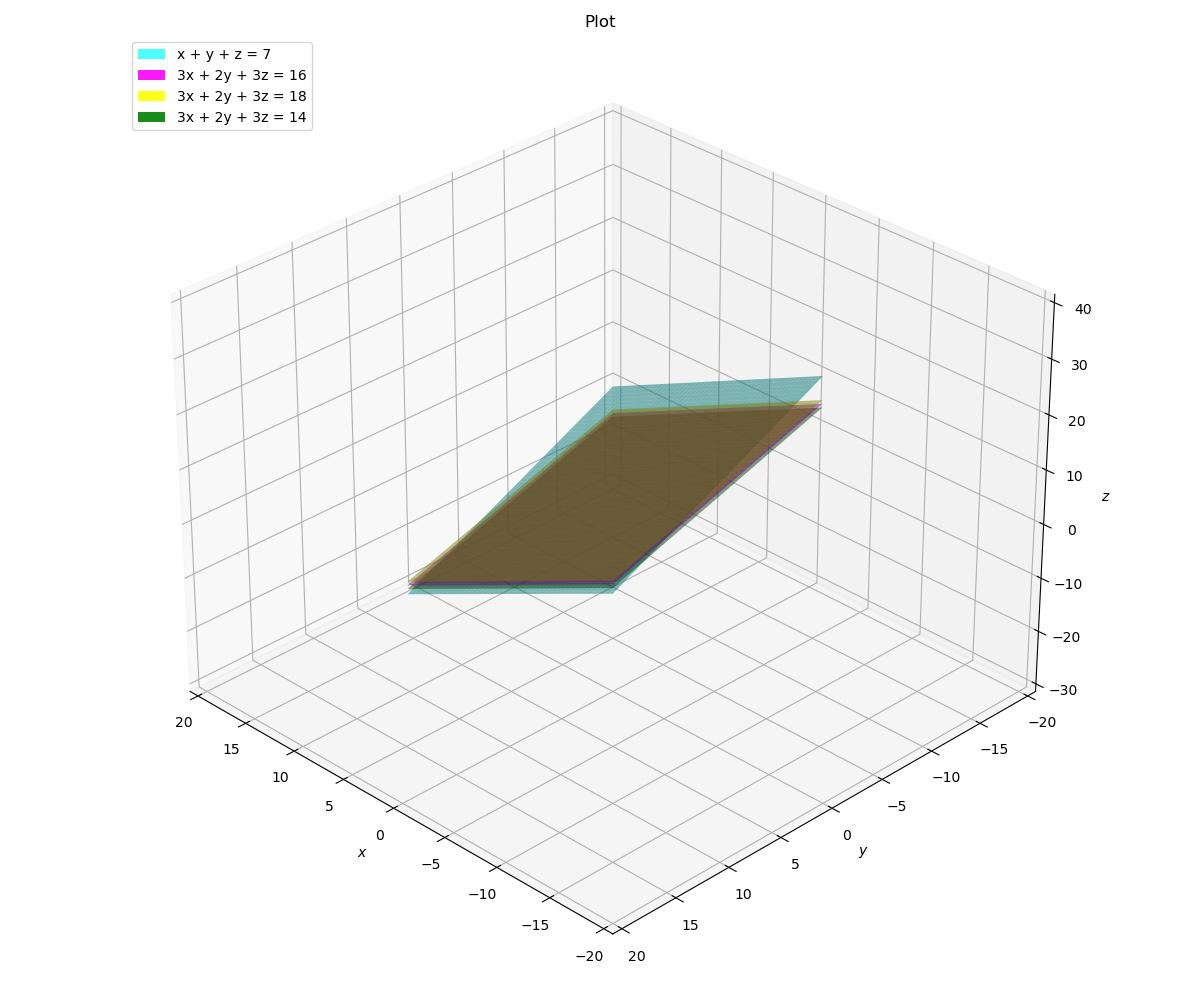
\includegraphics[width=0.5\columnwidth]{../figs/plot_p.jpg}
	\caption{Plot}
	\label{fig:fig}
\end{figure}
\end{frame}

\end{document}
